\scanpage{68}
% archive sheet number: 67

% L1–2, continuation
de la forme $g_*(G)$, où $g:\deleted{\unsure{\operatorname{Spec}}}x\longrightarrow X$, $G$ fini sur \deleted{$X$} $x$, \inserted{donc $\unsure{s|\nu|\varphi}(F)=\unsure{\varphi|\phi}(X)=\varphi(x)$} On a

% L3, spectral sequence
\[
H^*(\deleted{\unsure{k}}\unsure{k(x)|x|\overline{\{x\}}},G)\Longleftarrow H^p(X,R^q g_*(G))
\]

% L4, cancelled lemma
\deleted{\uline{Lemme} $R^qg_*(G)_{\unsure{z|2|\bar z}}\quad E_2^{pq}=0$ si $p+q>\varphi(x)$ et $q>0$.}

% L5–7, local ring and total fractions
Or pour $y\in X$, posant $\underline{\mathcal O}_{X,\bar y}={}$ anneau strict local au dessus de $y$ en $\bar y$, \deleted{\unsure{$R^q$|Rq.}} $K_{\bar y}=\underline{\mathcal O}_{X,\bar y}\otimes_X k(x)={}$ anneau total des fractions,

% L8–9, small square at left
\diagram{\begin{tikzcd}[ampersand replacement=\&,column sep=small,row sep=small]x\arrow[d]\&x_{\bar y}\arrow[l]\arrow[d]\\X\&X_{\bar y}\arrow[l]\end{tikzcd}}

% L8–12, stalk calculation
On aura $R^q g_*(G)_{\bar y}=H^q(K_{\bar y},G_{K_{\bar y}})$, \deleted{\unsure{donc}} qui est nul sauf si $q\leq\mathrm{cd}_l(K_{\bar y})$ ; donc (pour $q$ donné) les pts \deleted{$y$ en question, \unsure{on}} $y\in\operatorname{supp}R^q g_*(G)$ satisfont $\varphi(y)<\varphi(x)-\mathrm{cd}_l(K_{\bar y})\leq\varphi(x)-q$ \inserted{Condition b} d'où

% L13, boxed bound
\[
\boxed{s(R^qg_*(G))<\varphi(x)-q}\deleted{\unsure{\leq}}
\]

% L13–14, small text on left
D'autre part, si $q>0$, on a $R^q g_*(F)_x=0$, et l'hyp. de récurrence noeth. s'applique, donc

% L14–16, exceptional degrees
$H^p(X,R^qg_*(G))=0$ sauf pour $p\unsure{<|\leq}\varphi(x)-q\deleted{\unsure{2}}$ i.e. $p\unsure{-|+}q<\varphi(x)$, donc

% L16, vanishing range
\[
E_2^{pq}=0\quad\text{si}\quad p-q\geq\varphi(x),\quad q>0
\]

% L17–20, left degree diagram
\figure{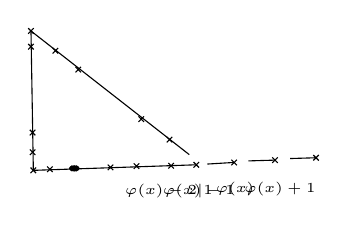
\begin{tikzpicture}[x=1cm,y=1cm]\draw (.02,1.77)--(.05,0)--(2.10,.07);\draw (.02,1.77)--(2.03,.20);\draw (2.26,.08)--(2.59,.10) (2.78,.12)--(3.12,.13) (3.31,.15)--(3.64,.16);
\foreach \x/\y in {.02/1.77,.02/1.57,.04/.48,.04/.23,.05/0,.26/.014,.57/.025,1.03/.037,1.36/.053,1.80/.058,2.12/.070,2.60/.10,3.12/.13,3.64/.16,.33/1.52,.62/1.28,1.42/.65,1.78/.39}{\draw (\x-.035,\y-.035)--(\x+.035,\y+.035) (\x-.035,\y+.035)--(\x+.035,\y-.035);}
\fill (.57,.025) ellipse (.07 and .04);
\node[below,font=\tiny] at (1.77,-.055) {$\varphi(x)-\unsure{2|1}$};\node[below,font=\tiny] at (2.15,-.055) {$\varphi(x)-1$};\node[below,font=\tiny] at (2.61,-.03) {$\varphi(x)$};\node[below,font=\tiny] at (3.18,-.03) {$\varphi(x)+1$};\end{tikzpicture}}

% L17–20, conclusion
La suite spectrale donne alors $H^{\unsure{n|*}}(X,g_*(G))\simeq H^n(x,G)$ pour $n\geq\varphi(x)+1$. Or, par l'hyp. a), le deuxième membre est nul, OK.
